\documentclass[12pt, a4paper]{article}

\usepackage[margin=1in]{geometry}
\usepackage{graphicx}
\usepackage{amsmath}
\usepackage{amssymb}
\usepackage{natbib}
\usepackage{hyperref}
\usepackage{float}
\usepackage{setspace}
\usepackage{caption}
\usepackage[utf8]{inputenc}

\hypersetup{
    colorlinks=true,
    linkcolor=blue,
    filecolor=magenta,      
    urlcolor=cyan,
    citecolor=blue,
}

\bibliographystyle{apalike}
\setcitestyle{authoryear,open={(},close={)}}

\onehalfspacing

\title{\textbf{Including Dynamics in a Network-Based Stochastic Multi-hazard Model: A Virtual Testbed for Volcanic Ashfall and Flood Risk Assessment}}
\author{Mark Bebbington\textsuperscript{1}, 
Alexandre Dunant\textsuperscript{2}, 
David Hart\textsuperscript{3}, 
Stuart Mead\textsuperscript{1}, 
Melody Whitehead\textsuperscript{1}}
\date{\today}

\begin{document}

\maketitle

\begin{abstract}
\noindent Complex multi-risk frameworks, particularly those involving volcanic and hydrological hazards, produce cascading impacts that significantly challenge Disaster Risk Management (DRM). This study introduces a dynamic, network-based stochastic model developed as a virtual testbed to simulate complex multi-hazard interactions. The testbed captures time-dependent processes, allowing for the investigation of immediate, short-term, and long-term impacts of volcanic ashfall on river flow dynamics within a complex multi-risk framework. We apply the model to the Rangitaiki and Tarawera river systems in New Zealand, simulating hydrological processes over a 365-day period with intermittent volcanic eruptions. The model explicitly accounts for ashfall-induced changes in catchment hydrology. Our results demonstrate how testbeds can be use to explore "what-if" cascading impacts scenarios, by providing a flexible, computationally efficient framework, offering crucial support for Disaster Risk Management and Climate Change Adaptation (CCA) planning in volcanic regions.
\end{abstract}

\noindent\textbf{Keywords:} Multi-hazard; cascade; network; temporal; volcanic ashfall; flood risk; virtual testbed; Disaster Risk Management (DRM); Climate Change Adaptation (CCA)

\hrule

\section*{Highlights}
\begin{itemize}
    \item A dynamic network framework is implemented as a virtual testbed for simulating cascading multi-risk scenarios.
    \item The testbed explores interactions between volcanic ashfall and river systems across multiple time scales.
    \item Stochastic simulation of hazards supports robust risk assessment for decision-making under uncertainty.
    \item The model provides a computationally efficient tool for "what-if" analysis to support DRM and CCA.
    \item The case study demonstrates significant cascading impacts of ashfall on flood risk in a complex environment.
\end{itemize}
\hrule

\section{Introduction}
Understanding the complex interactions between multiple natural hazards remains one of the significant challenges in Disaster Risk Management (DRM) and Climate Change Adaptation (CCA). Many large-scale disasters involve multiple hazards affecting the same region either simultaneously or in rapid succession before complete recovery from the initial impact (\citealp{Guha-Sapir2016}; \citealp{DesInventar2023}). These cascading impacts, where an initial event triggers a sequence of subsequent hazards, create complex multi-risk frameworks that are difficult to predict and manage (\citealp{Liu2016}).

To address this challenge, the scientific community is moving towards the development of virtual testbeds within a comprehensive digital ecosystem. Such testbeds aim to simulate complex multi-risk processes in realistic virtual environments, serving as laboratories for improving the understanding of cascading impacts and for testing mitigation and adaptation strategies through "what-if" scenarios. This paper contributes to the conceptualization and implementation of such a testbed.

Volcanic regions are prime examples of complex multi-hazard environments. Historical eruptions demonstrate the potential for widespread impacts extending far beyond the immediate vicinity of the volcano. For example, the Taupo eruption of c. 186 AD dispersed vast quantities of ash over thousands of square kilometers in New Zealand's Taupo Volcanic Zone (TVZ) (\citealp{Wilson1985}). This widespread ashfall has the potential to trigger cascading hazards by interacting with other natural processes, most notably the hydrological cycle. A critical knowledge gap remains in our understanding of the dynamic interactions between volcanic ashfall and hydrological systems, which can lead to catastrophic compound events (\citealp{Gran2006}; \citealp{Gran2011}).

Previous research has advanced the conceptual understanding of multi-hazard interactions (\citealp{Gill2014}; \citealp{DeAngeli2022}), but often lacked the dynamic temporal elements required for realistic simulation. While recent network-based models have shown promise (\citealp{Dunant2021a}; \citealp{Dunant2021b}; \citealp{Dunant2025}), they have generally been static, limiting their ability to capture the evolving nature of cascading processes. To address these limitations, we propose a novel network-based stochastic multi-hazard model designed as a virtual testbed. Our approach incorporates dynamic temporal characteristics into a multi-risk framework, allowing for the realistic simulation of cascading events over time. Holme and Saramaki (2012) introduced the concept of time dependent networks and provided an overview of methods and applications. They argued that many real-world networks, such as social networks (Java et al., 2007; Cattuto et al., 2010), Saram¨aki, 2011), and biological networks (Han et al., 2004; Pascual & Dunne, 2006), are inherently dynamic and change over time, and that traditional network modelling methods may not be sufficient to capture their complexity and dynamics. 

By combining computationally efficient models for individual hazards and their interactions, we enable robust stochastic simulation over extended periods, providing a powerful tool for risk assessment and decision support.

\section{Study Area and Data}
The model is applied to the Rangitaiki and Tarawera river systems in the Bay of Plenty region of New Zealand’s North Island. These river systems drain the eastern side of the Taupo Volcanic Zone (TVZ), a highly active volcanic region that has experienced numerous eruptions throughout the Holocene (\citealp{Nairn2002}). The combination of active volcanism and flood-prone river systems makes this region an ideal case study for investigating cascading hazards. The study area, including the delineated catchments and the network model structure consisting of nodes (reaches) and edges (connections), is shown in Figure \ref{fig:study_area}.

Catchment and river network characteristics were extracted from a 25-meter resolution digital elevation model (DEM) using the `pyflwdir and networkX` library. This provided the spatial framework for the model, including river segment locations, catchment boundaries, area, and slope. The volcanic source for ashfall simulations was located at coordinates (1852398, 5703897) in the local projection, location of the Taupo volcanic field. It is important to note, in the context of testbed herein, that any raster file and volcano location can be used allowing for testing of different geomorphological settings.

\begin{figure}[H]
    \centering
    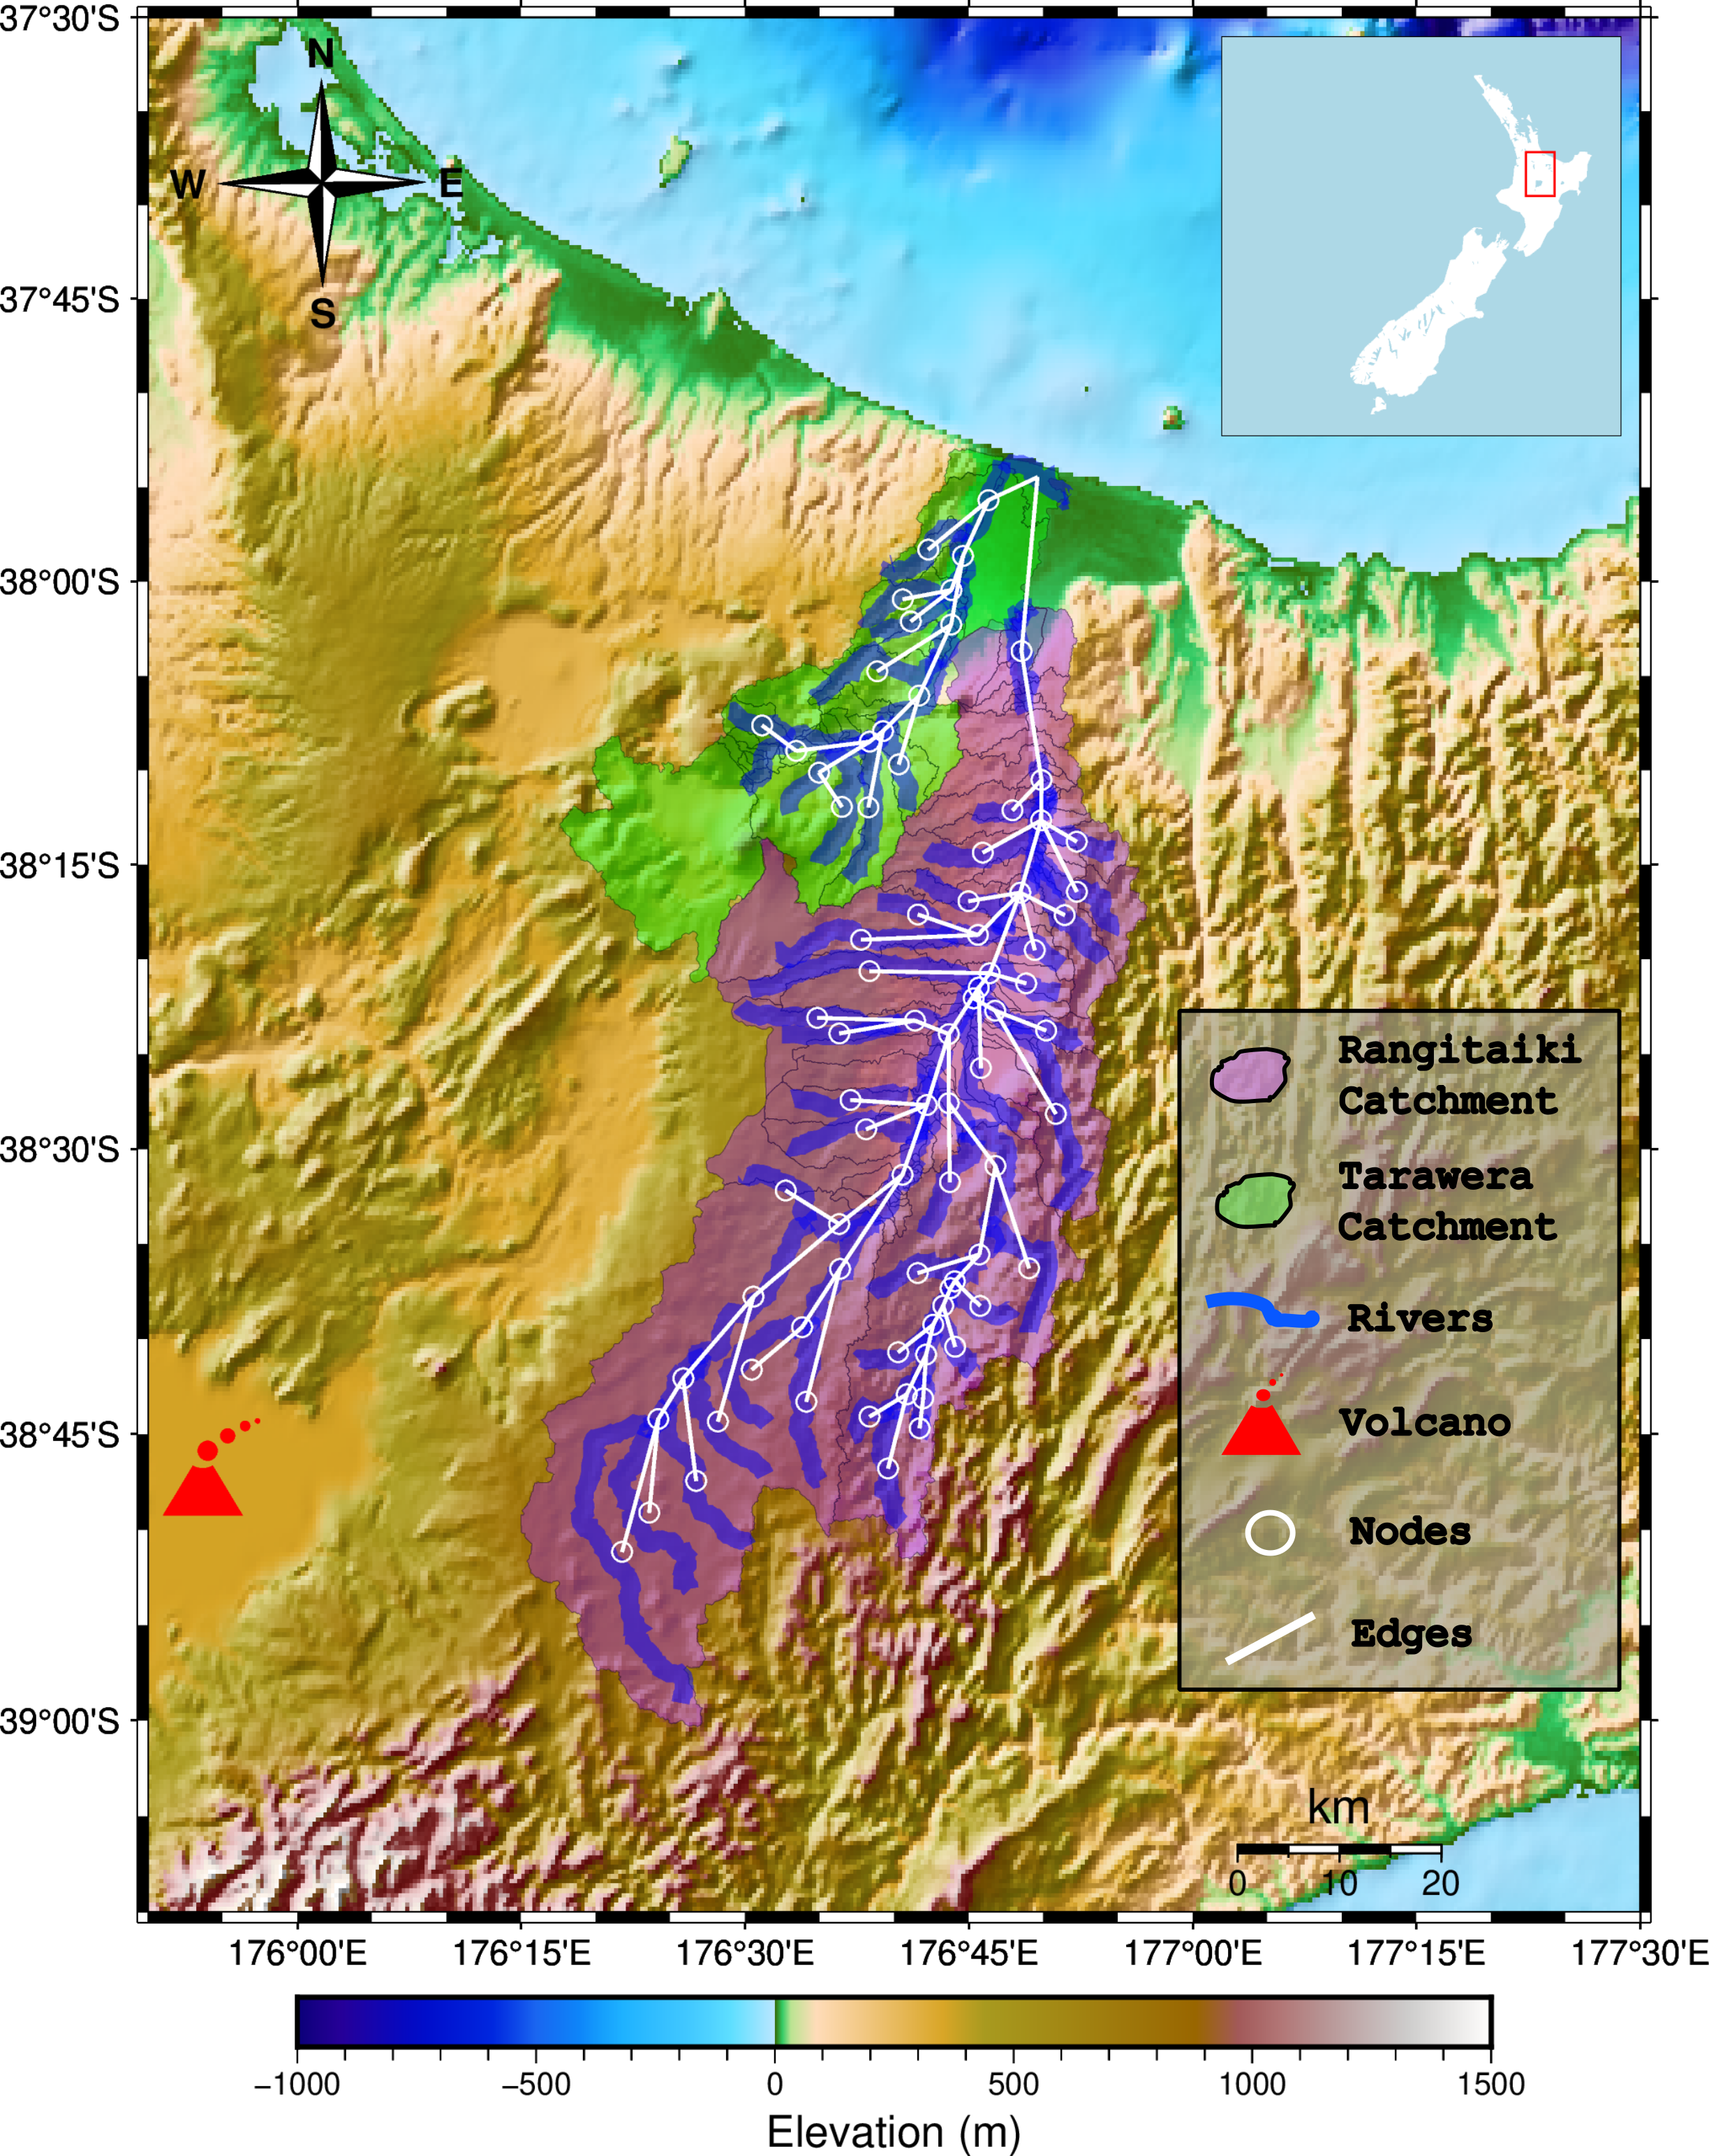
\includegraphics[width=1\linewidth]{network.png}
    \caption{Map of the study area showing the Rangitaiki and Tarawera river systems in relation to the local topography and the Taupo Volcanic Zone. The model's network structure, consisting of nodes (river reaches) and edges (downstream connections), is overlaid on the catchments. The location of the volcanic source for ashfall simulations is also indicated.}
    \label{fig:study_area}
\end{figure}


\section{Methodology}
The virtual testbed is built upon a modular framework where each component simulates a specific physical process on an hourly time step. The overall architecture is designed to capture the cascading effects from volcanic ash deposition to altered hydrological response and subsequent sediment transport. An overview of the algorithm is summarized in Figure \ref{fig:flowchart}.

\begin{figure}[H]
  \centering
  % limit to 0.6\linewidth wide and 0.3\textheight tall, but don't distort
  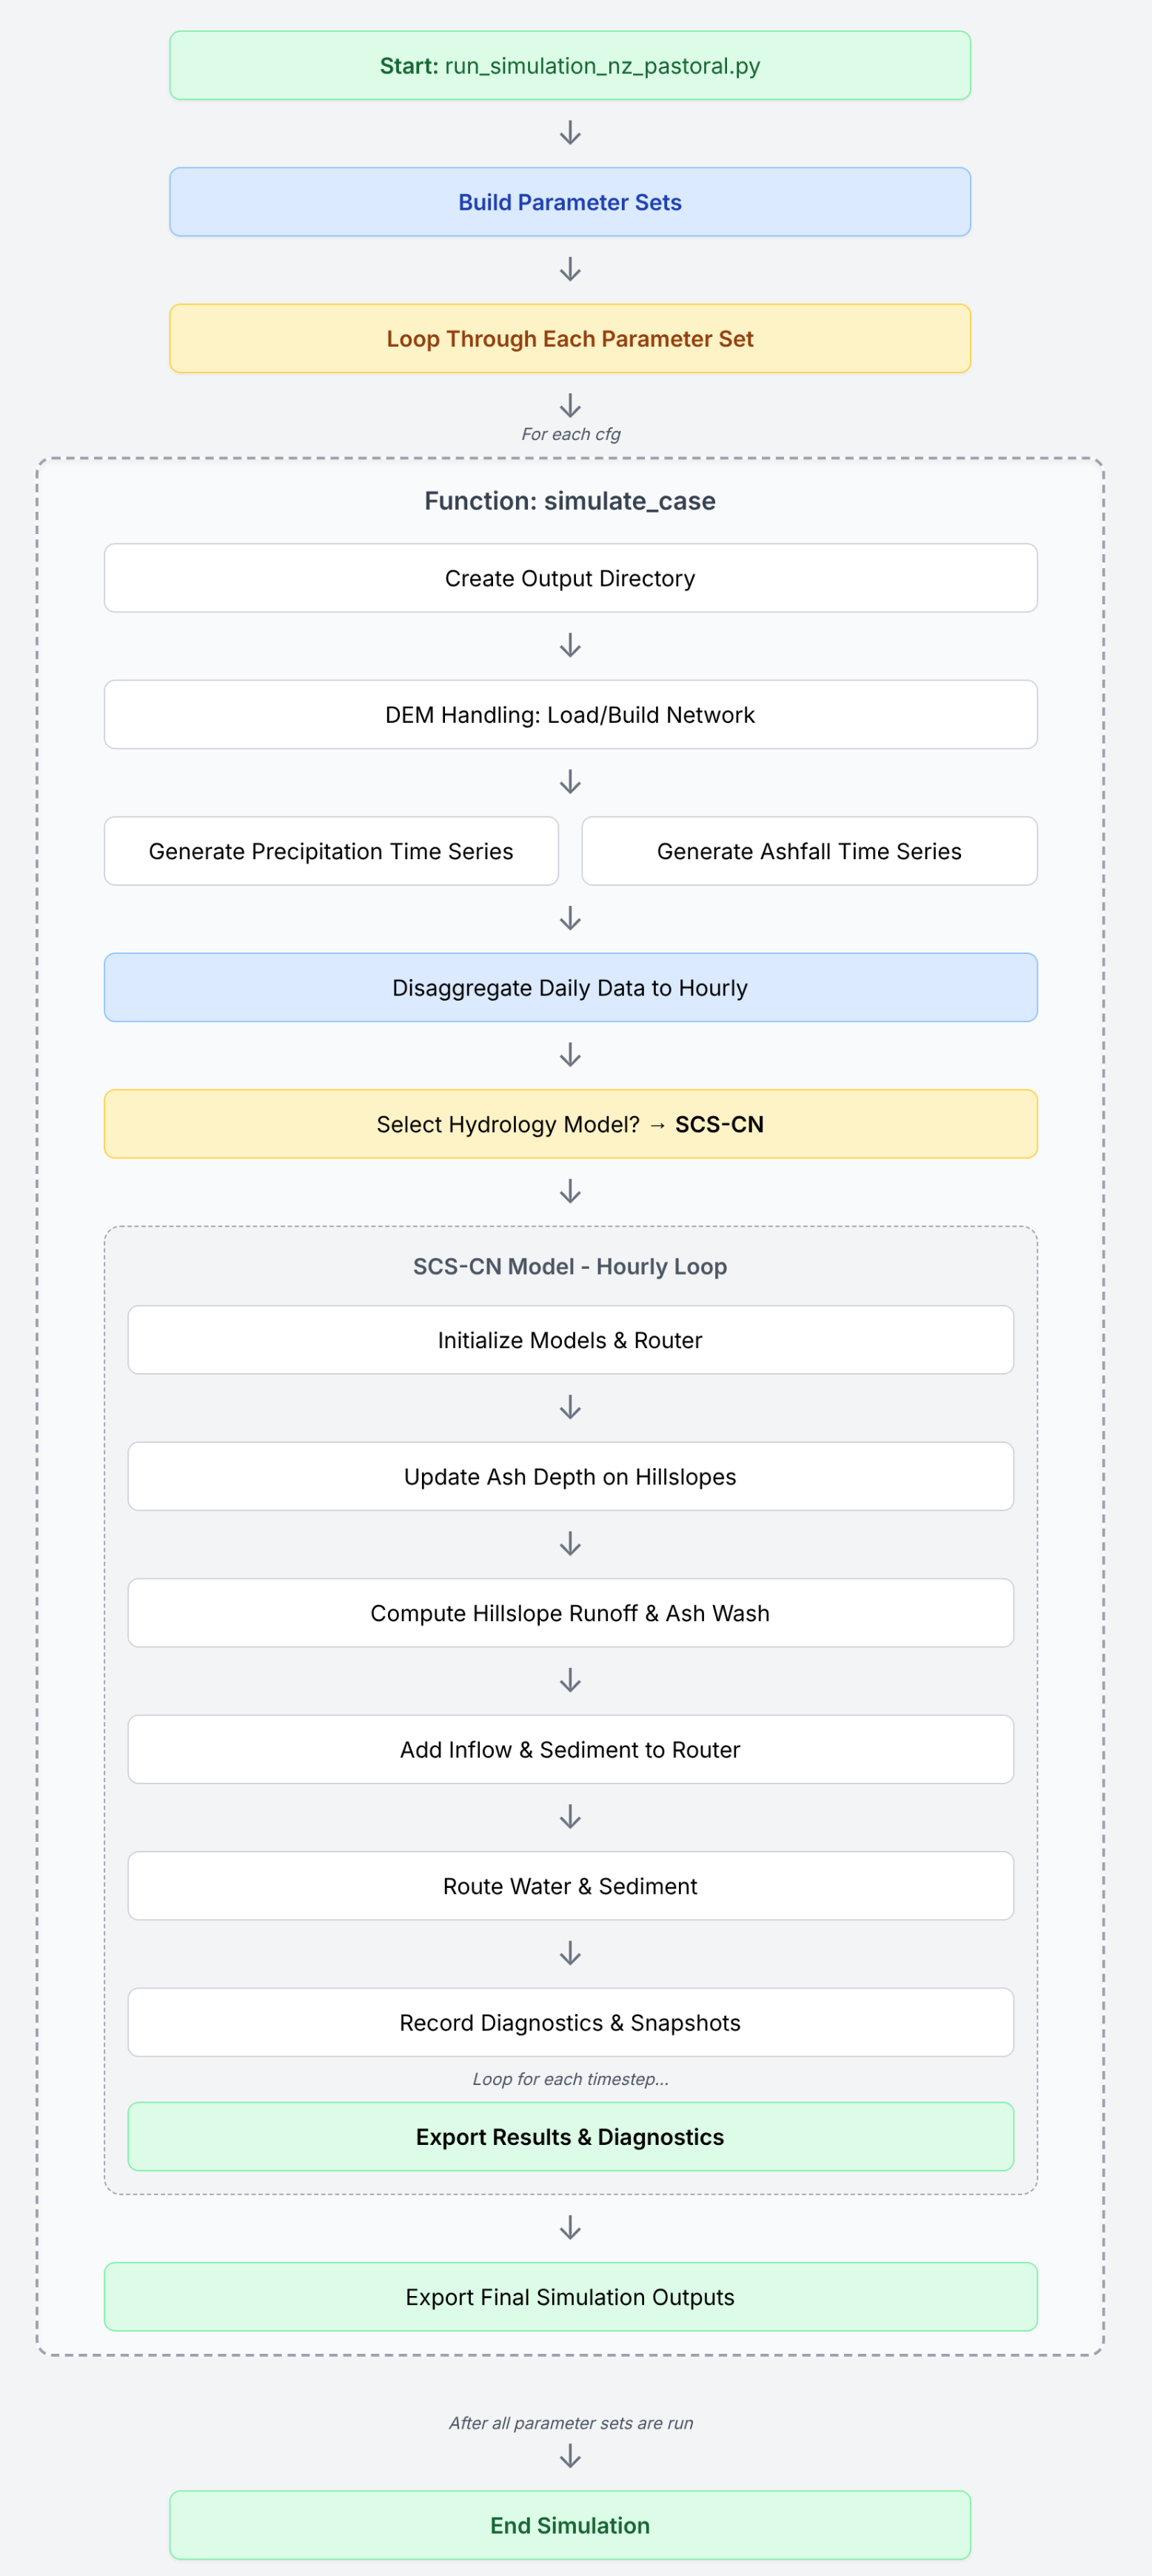
\includegraphics[width=0.5\linewidth,height=0.7\textheight]{diagram.png}
  \caption{Algorithm flowchart}
  \label{fig:flowchart}
\end{figure}


\subsection{River Network and Catchment Delineation}
The spatial foundation of the model is a digital elevation model (DEM) of the study area. Using the `pyflwdir` library, the DEM is processed to derive flow directions, stream order, and sub-catchment boundaries. A river network is extracted by defining a minimum threshold for stream order (Strahler order $\ge 8$). This network is then topologically cleaned, using the `networkX` library, to remove disconnected components and cycles, resulting in a directed acyclic graph where each node represents a river reach and each edge represents a downstream connection (Figure \ref{fig:study_area}). This process ensures that water and sediment can be efficiently routed from the headwaters to the outlet. The DEM, if missing, can also be loaded based on a coordinates bounding box, from the 'pyGMT' library.

\subsection{Stochastic Hazard Models}

\subsubsection{Stochastic Precipitation Model}
The model is driven by a stochastic precipitation generator that produces hourly rainfall data for the entire simulation period. Daily rainfall depth is first drawn from a Gamma distribution to account for the skewed nature of precipitation events. Intermittency (dry days) is introduced via a daily rain probability (`rain-prob` = 0.5). To capture seasonal patterns, a sinusoidal function modulates the daily rainfall totals over the year, controlled by a `season-strength` parameter. Finally, the generated daily precipitation is uniformly disaggregated into hourly values to be used in the hydrological model.

\subsubsection{Volcanic Ashfall Simulation}

Intermittent volcanic eruptions, which act as the primary trigger for the cascading hazard sequence, are simulated using a flexible stochastic framework. The model offers two distinct modes for determining the timing of eruptive events to accommodate different research objectives:
\begin{enumerate}
    \item \textbf{Stochastic Renewal Process:} For long-term probabilistic risk assessment, the time between eruptions can be modeled as a renewal process following a Weibull distribution. This is controlled by the \texttt{weibull\_shape} and \texttt{weibull\_scale} parameters, allowing for the simulation of eruption patterns with varying degrees of regularity.
    \item \textbf{Deterministic Scenario:} For hindcasting specific historical events or exploring predefined "what-if" scenarios, the model can accept a \texttt{predefined\_eruptions\_list}. This allows the user to specify the exact days on which eruptions occur during the simulation.
\end{enumerate}

When an eruption is triggered, its magnitude and dispersal characteristics are determined stochastically. First, a magnitude event, \(M_0\), is drawn from a uniform distribution defined by \texttt{min\_magnitude} and \texttt{max\_magnitude}. This value then scales the parameters of the tephra fall model, which is based on the work of \citet{Gonzalez-Mellado2010}. The resulting tephra thickness, \(T\) (in cm), at any given point on the landscape is calculated as:

\begin{equation}
    T(d, \theta) = \gamma_{\text{eff}} \cdot \exp[-\beta_u d(1-\cos(\theta - \phi))] \cdot d^{-\alpha_{\text{eff}}}
    \label{eq:ashfall}
\end{equation}

The parameters of this equation are defined as follows:
\begin{itemize}
    \item \(d\) and \(\theta\): These are the geometric coordinates of a location relative to the volcanic vent, representing the distance (in km) and the angle (in radians), respectively.
    \item \(\gamma_{\text{eff}}\): The effective eruption size parameter, which controls the overall volume of tephra. It is scaled directly by the eruption magnitude \(M_0\) and a baseline coefficient \(\gamma_0\):
    \begin{equation}
        \gamma_{\text{eff}} = \gamma_0 \cdot 10^{M_0}
    \end{equation}
    \item \(\alpha_{\text{eff}}\): The effective distance-decay exponent, which governs how quickly the ash deposit thins with distance from the source. This parameter is inversely related to magnitude, reflecting the wider dispersal of larger eruptions, and is scaled by a baseline exponent \(\eta_0\):
    \begin{equation}
        \alpha_{\text{eff}} = \frac{\eta_0}{M_0 + 1}
    \end{equation}
    \item \(\phi\): The main dispersal axis, representing the dominant wind direction. This is determined stochastically for each eruption by drawing a value from a uniform distribution bounded by \texttt{wind\_dir\_min} and \texttt{wind\_dir\_max} (in degrees).
    \item \(\beta_u\): A parameter that controls the shape of the deposit and the influence of wind on its elongation. This is typically set as a constant for a given region or eruption type.
\end{itemize}

The complete set of user-configurable parameters for the volcanic ashfall simulation provides a high degree of flexibility for scenario testing:
\begin{itemize}
    \item \texttt{use\_predefined\_eruptions}: (Boolean) Switches between stochastic and deterministic eruption timing.
    \item \texttt{predefined\_eruptions\_list}: (List of integers) Specifies eruption days if the above is true.
    \item \texttt{weibull\_shape}, \texttt{weibull\_scale}: (Floats) Parameters for the Weibull distribution of inter-eruption times.
    \item \texttt{min\_magnitude}, \texttt{max\_magnitude}: (Floats) Defines the range for the stochastic eruption magnitude, \(M_0\).
    \item \texttt{gamma0} (\(\gamma_0\)), \texttt{eta0} (\(\eta_0\)): (Floats) Baseline coefficients for scaling tephra volume and dispersal.
    \item \texttt{wind\_dir\_min}, \texttt{wind\_dir\_max}: (Floats) Defines the range for the stochastic wind direction, \(\phi\).
    \item \texttt{beta\_u} (\(\beta_u\)): (Float) The wind influence/deposit shape parameter.
\end{itemize}

Once the total ashfall depth for each catchment is calculated, it is uniformly disaggregated to an hourly rate, providing the necessary input for the time-step-based hydrological and sediment transport models. This detailed, parameter-driven approach allows the virtual testbed to explore a wide range of potential volcanic activities and their cascading impacts on the river system.

\subsection{Hydrological Response and Ash Mobilization}

\subsubsection{Runoff Generation: SCS-CN with Ash Impact}
The core of the hydrological simulation is an hourly SCS Curve Number (SCS-CN) model for each catchment. This method calculates runoff based on precipitation, soil type, and land use (\citealp{USDA1986}). The potential maximum soil moisture retention, $S$ (in inches), is calculated from a baseline Curve Number ($\text{CN}_{\text{base}}$):

\begin{equation}
S_{\text{base}} = \frac{1000}{\text{CN}_{\text{base}}} - 10
\end{equation}

Runoff is generated only after an initial abstraction, $I_a$, which represents interception and surface storage. $I_a$ is modeled as a fraction ($\lambda$) of $S$:

\begin{equation}
I_a = \lambda S
\end{equation}

For this study, $\lambda$ was set to 0.05, a value more representative of wet, temperate pastoral lands than the standard value of 0.2.

A key innovation in the model is the dynamic impact of ashfall on runoff generation, which represents the physical process of soil sealing illustrated in Figure \ref{fig:sealing}. The presence of ash reduces infiltration by increasing the effective Curve Number ($\text{CN}_{\text{eff}}$). This effect is parametrized as a function of ash thickness, $h_{\text{ash}}$ (in mm), and an `ash-cn-multiplier` ($m_{\text{CN}}$), which amplifies the hydrological sensitivity to thin ash layers:

\begin{equation}
\Delta_{\text{CN}} = \min(5, h_{\text{ash}} \cdot m_{\text{CN}})
\end{equation}
\begin{equation}
\text{CN}_{\text{eff}} = \min(98, \text{CN}_{\text{base}} + \Delta_{\text{CN}})
\end{equation}

The runoff depth, $Q_{\text{runoff}}$ (in mm), for a given hourly precipitation, $P$ (in mm), is then calculated using the effective retention, $S_{\text{eff}}$ (derived from $\text{CN}_{\text{eff}}$):

\begin{equation}
Q_{\text{runoff}} = \frac{(P - I_a)^2}{P - I_a + S_{\text{eff}}} \quad \text{for } P > I_a
\end{equation}


\begin{figure}[H]
    \centering
    \includegraphics[width=0.8\linewidth]{sealing.png}
    \caption{Conceptual illustration of the primary cascading impact mechanism modeled. \textbf{(A)} In pre-disturbance conditions, precipitation is partitioned into interception, infiltration, and overland flow. \textbf{(B)} Following a volcanic eruption, a tephra-fall layer blankets the ground, sealing soil pores. This significantly reduces infiltration and increases the proportion of precipitation that becomes overland flow, leading to faster and larger flood peaks (modified from \citealp{Pierson2014}).}
    \label{fig:sealing}
\end{figure}

\subsubsection{Hydrograph Generation and Routing}
The hourly runoff volume from each catchment is converted into a discharge hydrograph by convolution with a triangular Unit Hydrograph (UH). The shape of the UH is determined by the catchment's time of concentration, $t_c$ (in hours), which is calculated using the Giandotti formula (\citealp{Chow1988}):

\begin{equation}
t_c = \frac{4\sqrt{A} + 1.5L}{0.8\sqrt{H}}
\end{equation}

where $A$ is the catchment area (km$^2$), $L$ is the main channel length (km), and $H$ is the total elevation drop (m). The UH parameters—time to peak ($t_p$), time base ($t_b$), and peak discharge per unit of runoff ($q_p$)—are derived directly from $t_c$ as implemented in the \texttt{SCSCN\_UH\_Model} class:

\begin{gather}
t_p = 0.6 \cdot t_c \\
t_b = 2.67 \cdot t_p \\
q_p = \frac{0.208 A}{t_p}
\end{gather}

The generated hydrographs from all headwater catchments are introduced as lateral inflows to their corresponding river reaches. The hydrographs are then routed through the river network using a lag-based system implemented in the \texttt{NetworkRouterWithSediment} class. This approach translates the flow downstream, accounting for the travel time in each river reach, which is calculated based on the reach length and a defined \texttt{channel\_velocity\_ms} parameter.

\subsubsection{Hillslope Wash Model}
Ash accumulated on the catchment surface is mobilized and washed into the river network. This process is driven by the incremental runoff generated in each time step. The mass of ash available on the hillslope ($M_{\text{avail}}$) is tracked based on its density, area, and current thickness.

The mass of ash washed into the river during one time step ($M_{\text{wash}}$) is modelled as a fraction of the available mass, proportional to the runoff depth. This is governed by a \texttt{wash\_efficiency} parameter ($\eta_{\text{wash}}$) and the incremental runoff depth ($Q_{\text{runoff}}$) for the current step, as implemented in the \texttt{compute\_ash\_wash} function. The potential mass to be washed is calculated as:

\begin{equation}
M_{\text{wash, pot}} = M_{\text{avail}} \cdot \eta_{\text{wash}} \cdot \left( \frac{Q_{\text{runoff}}}{\Delta Q_{\text{ref}}} \right)
\end{equation}

where $\Delta Q_{\text{ref}}$ is a reference runoff depth (e.g., 10 mm) used to keep the efficiency parameter dimensionless (mm/mm). The actual mass washed is then limited by the total mass available:

\begin{equation}
M_{\text{wash}} = \min(M_{\text{avail}}, M_{\text{wash, pot}})
\end{equation}

This approach ensures that erosion events are directly coupled with the magnitude of the generated surface runoff in each time step.

\subsubsection{In-Stream Sediment (Ash) Transport}
Once in the river, ash is treated as sediment, and its transport is governed by the hydraulic conditions in each reach, managed by the \texttt{Reach} and \texttt{DCascade} classes. The transport capacity is based on bed shear stress, $\tau$, which is calculated for each reach at each time step and inspired by the D-cascade framework (\citealp{Tangi2022}) and its mass balancing approach (i.e. mobilisation and deposition downstream based on flow capacity):

\begin{equation}
\tau = \rho_w g R_h S_0
\end{equation}

where $\rho_w$ is the density of water, $g$ is gravitational acceleration, $S_0$ is the channel slope, and $R_h$ is the hydraulic radius. A key dynamic component is that the hydraulic radius is computed at each step as a function of the current discharge ($Q$) and channel width ($W$), making the transport capacity highly responsive to flow conditions. The ash transport capacity for the reach, $T_c$ (in kg per time step), is modelled as a power-law function of the shear stress, scaled by a \texttt{transport\_coefficient} ($k_t$), channel width ($W$), and length ($L$):

\begin{equation}
T_c = k_t \cdot (\tau^{1.5}) \cdot W \cdot L
\end{equation}

The mass of ash exported from a reach is the minimum of the ash available in storage within that reach and its calculated transport capacity, $T_c$. The routing of sediment through the network is performed using the topological backbone of the river graph to ensure mass conservation from upstream to downstream reaches. The  current model is a simplified version of the D-cascade framework (\citealp{Tangi2022}) as it considers only a uniform sediment class, a "mixed" reservoir model (i.e. not stratified), the sediment delivery is from node to node and the river network geomorphology is considered static.

\subsection{Simulation Design}
A single, detailed simulation was conducted for a 365-day period to analyze the stock-and-flow dynamics of the coupled system. The simulation was run on an hourly time step using the \texttt{scscn} model configuration. The parameters were chosen to represent a typical pastoral land-use scenario in New Zealand's North Island, as specified in the simulation configuration file. Key parameters include:
\begin{itemize}
    \item \textbf{Hydrology:} \texttt{curve\_number} = 70, \texttt{initial\_abstraction\_ratio} = 0.05, \texttt{channel\_velocity\_ms} = 0.5.
    \item \textbf{Precipitation:} \texttt{mean\_annual\_precip} = 2500 mm/year, \texttt{rain\_prob} = 0.5, \texttt{season\_strength} = 0.2.
    \item \textbf{Ash Impact:} \texttt{max\_cn\_increase} = 25.0, \texttt{k\_ash} = 0.5.
    \item \textbf{Ash Transport:} \texttt{wash\_efficiency} = 0.05, \texttt{transport\_coefficient} = 5e-4, \texttt{rho\_ash} = 1000.0 kg/m$^3$.
    \item \textbf{Eruption Scenario:} A single eruption of magnitude \texttt{M0} = 4.0 was configured to occur on day 180 of the simulation (\texttt{eruption\_days} = [180]).
\end{itemize}

\section{Results}
The simulation results provide a detailed picture of the dynamic, cascading interactions between volcanic ashfall, rainfall, and river system response. We focus on the stock-and-flow relationship, which describes how ash (stock) is stored in and released from the catchment and river network in response to hydrological events (flow).

\subsection{Ash Stock and Flow Dynamics}
The 365-day simulation included a significant eruption event on day 180. Figure \ref{fig:stockflow}, generated directly from the simulation outputs, presents the core results, illustrating the relationship between hydrological drivers, sediment fluxes, and sediment stocks.




\begin{figure}[H]
    \centering
    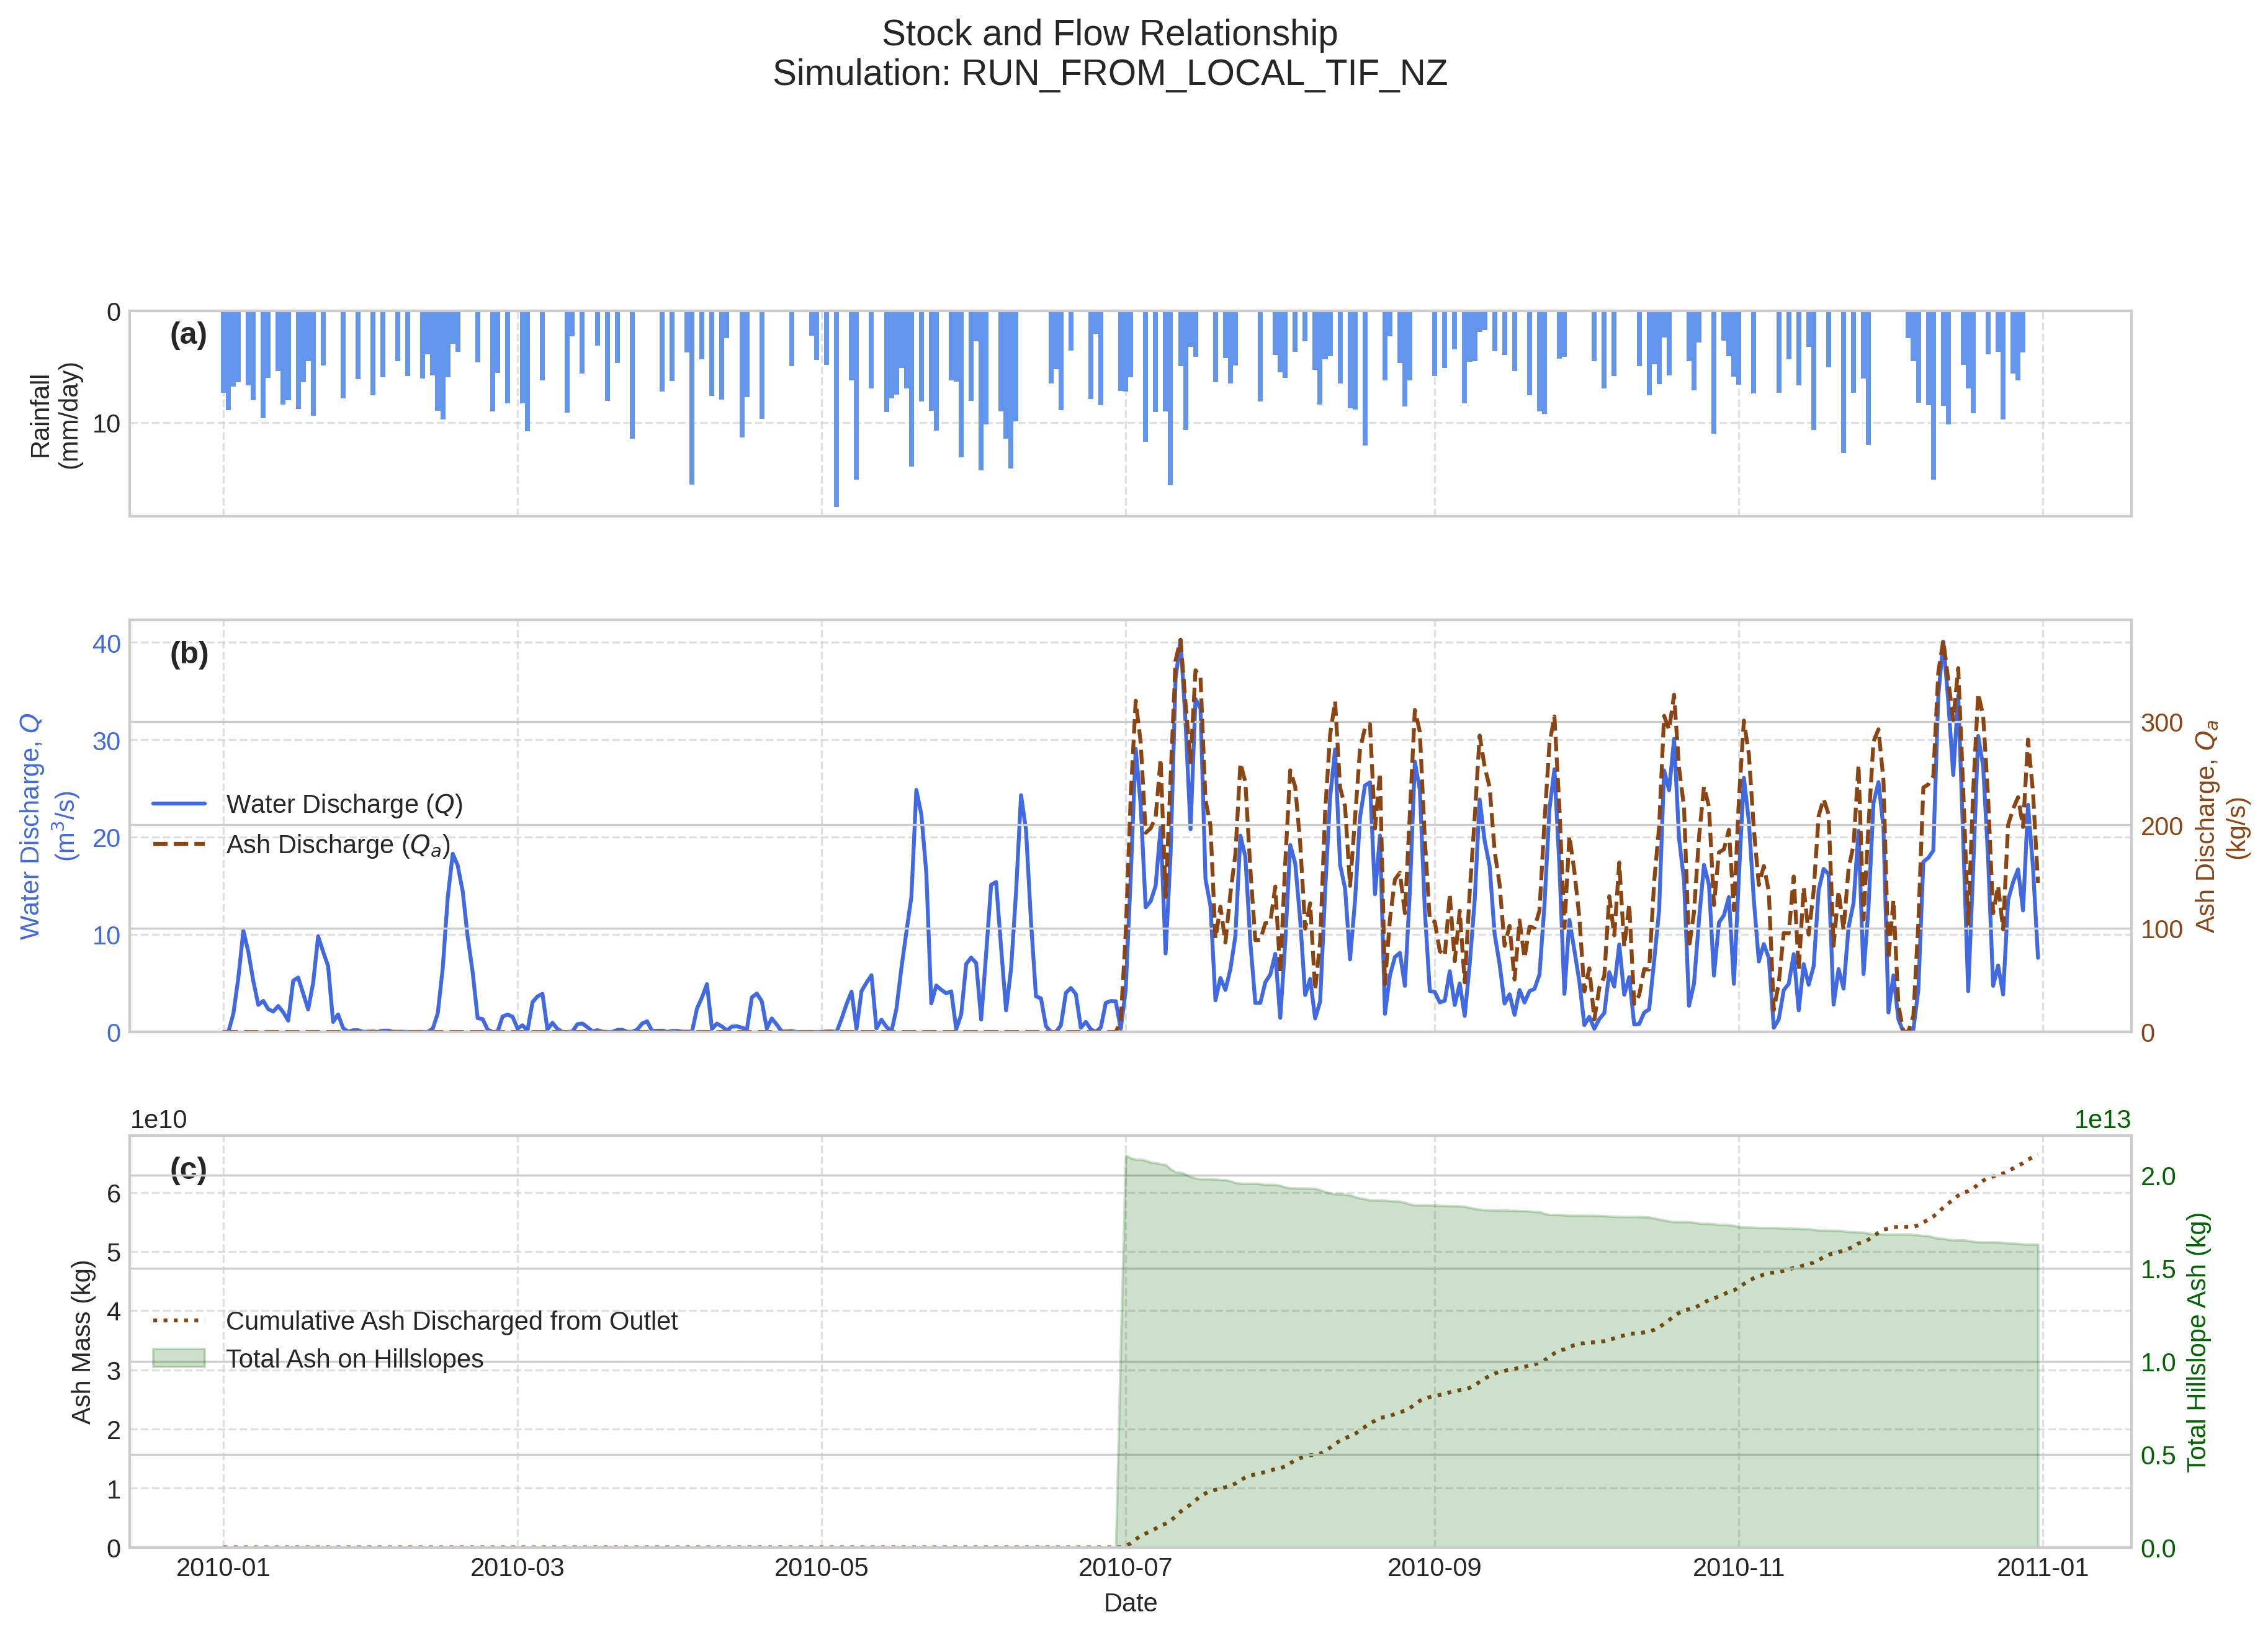
\includegraphics[width=1\linewidth]{stock_flow.png}
    \caption{Stock and flow relationship for the 365-day simulation. \textbf{(a)} Daily rainfall driving the system. \textbf{(b)} "Flows" at the network outlet, showing water discharge (Q, blue) and ash discharge (Qa, brown dashed). \textbf{(c)} "Stocks," showing the cumulative mass of ash washed from hillslopes into the river network (green dotted) and the total mass of ash concurrently stored within the river channels (purple).}
    \label{fig:stockflow}
\end{figure}


\begin{figure}[H]
    \centering
    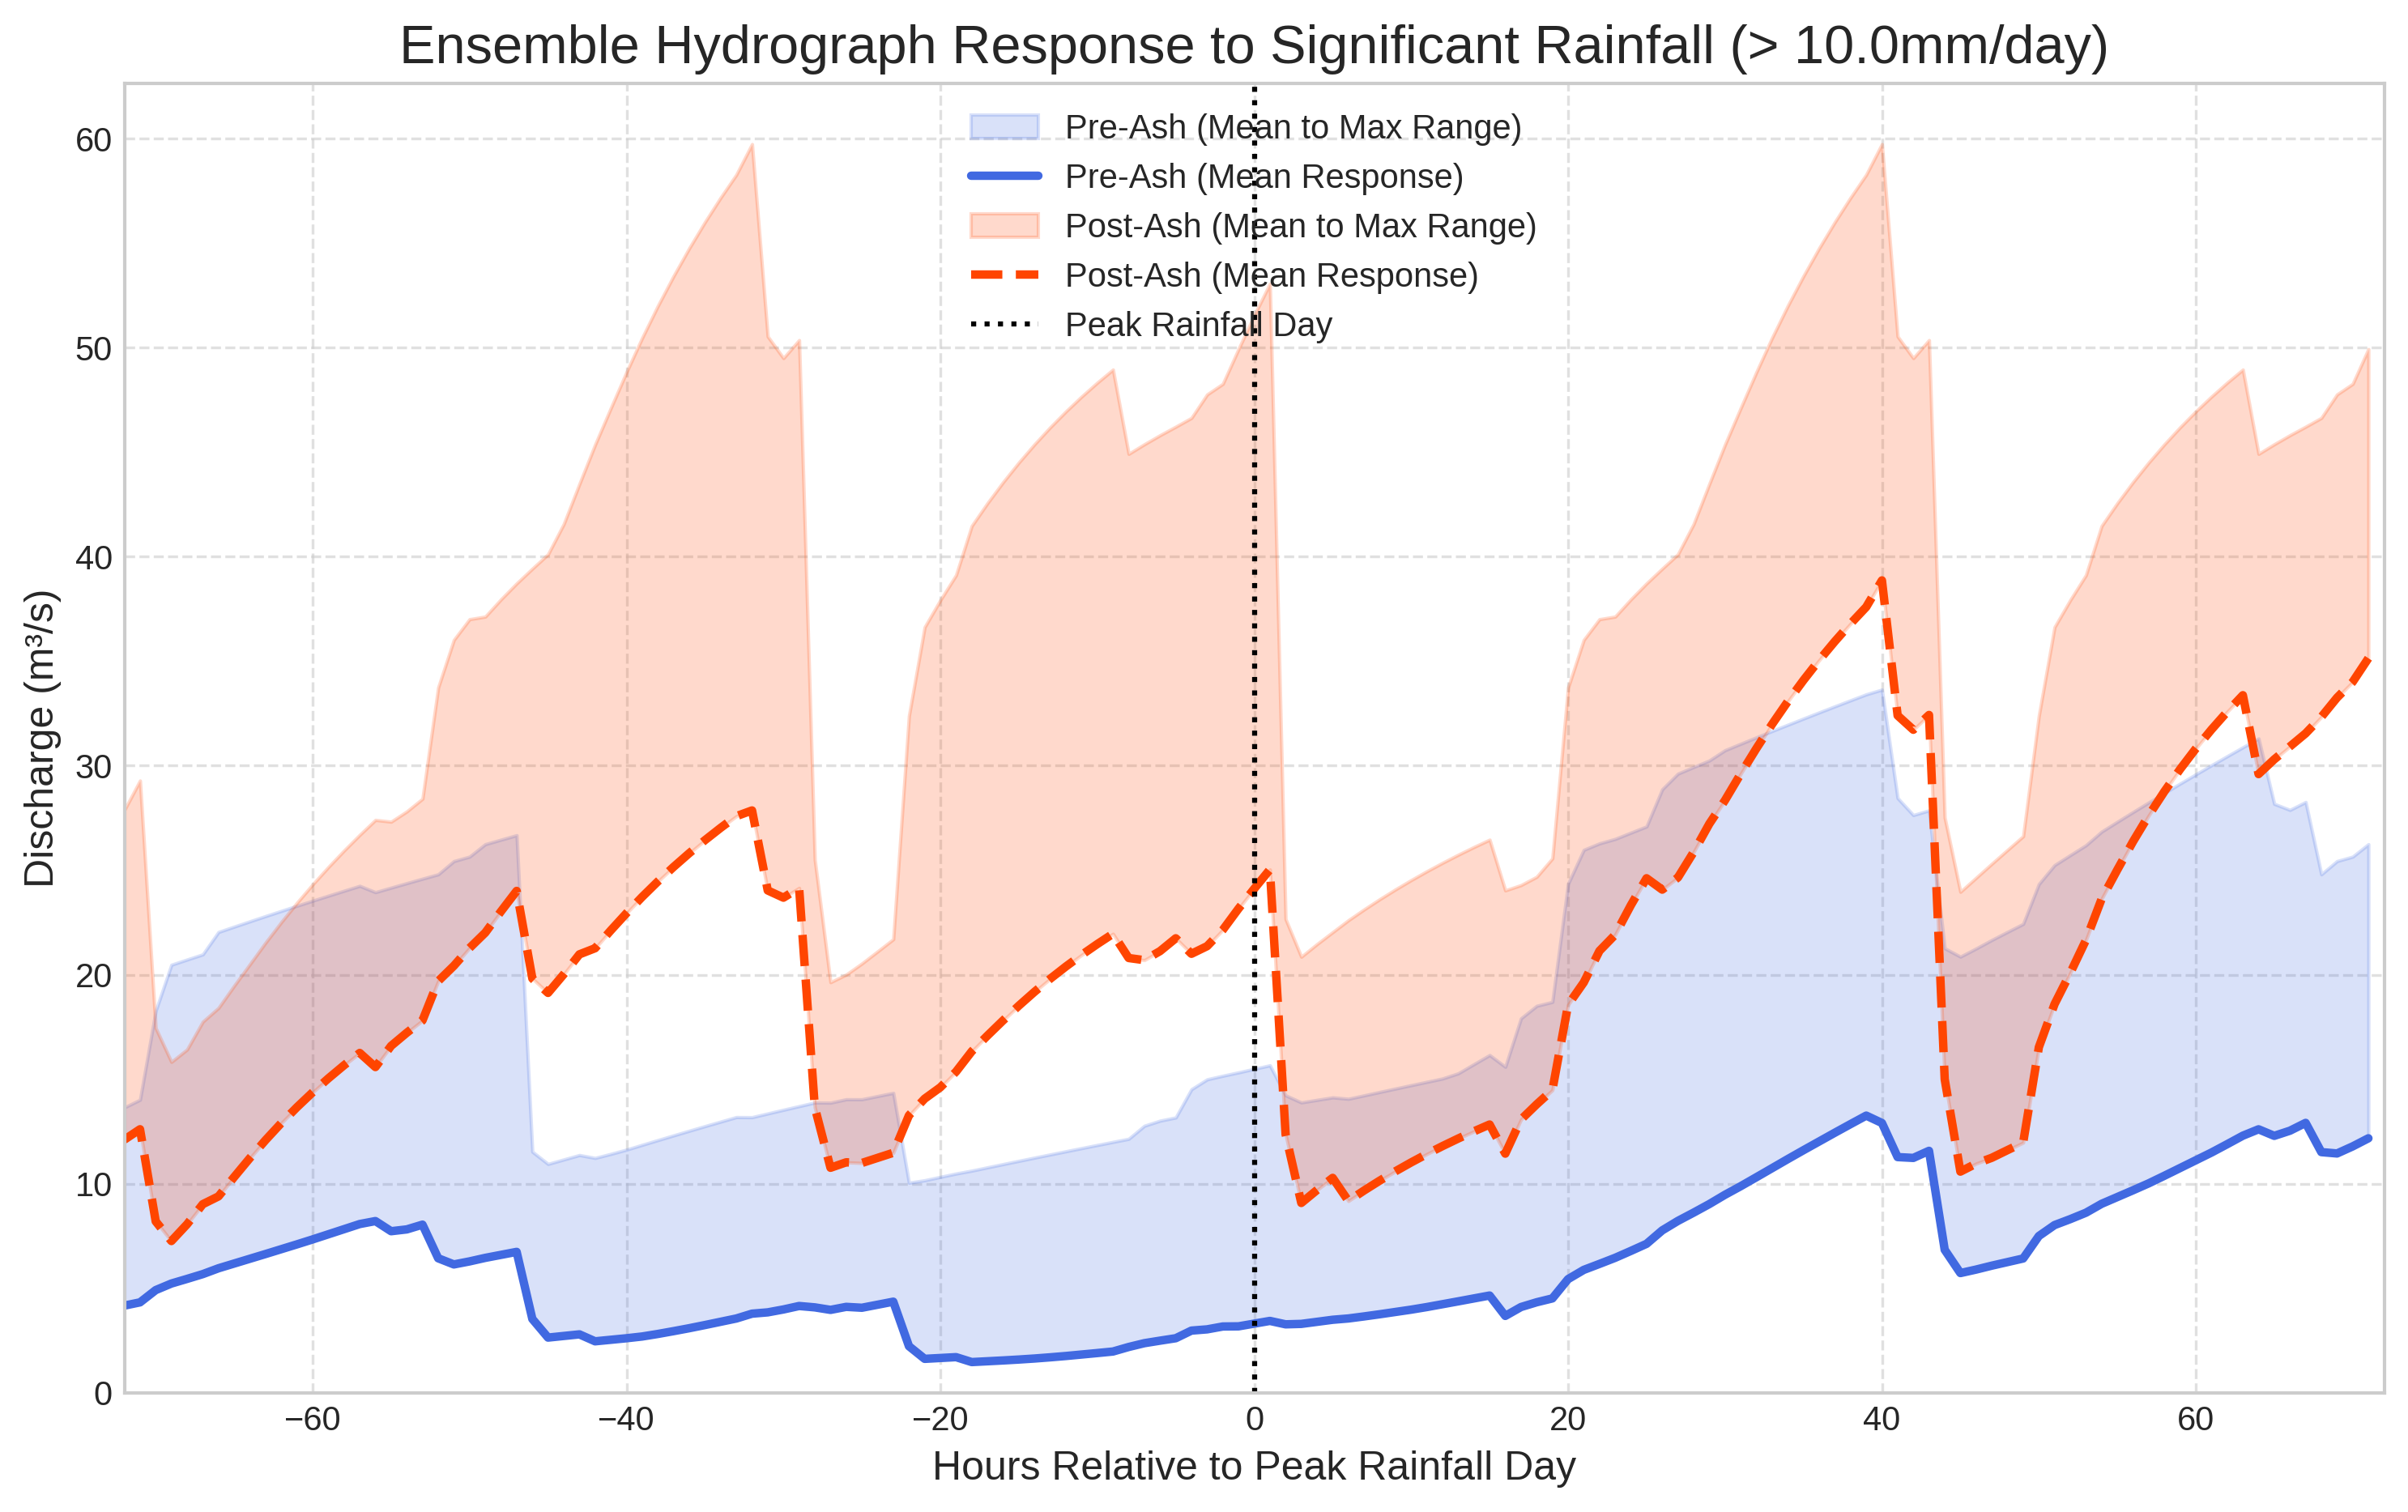
\includegraphics[width=1\linewidth]{hydrograph_ensemble.png}
    \caption{Stock and flow relationship for the 365-day simulation. \textbf{(a)} Daily rainfall driving the system. \textbf{(b)} "Flows" at the network outlet, showing water discharge (Q, blue) and ash discharge (Qa, brown dashed). \textbf{(c)} "Stocks," showing the cumulative mass of ash washed from hillslopes into the river network (green dotted) and the total mass of ash concurrently stored within the river channels (purple).}
    \label{fig:hydrograph_ensemble}
\end{figure}


Panel (a) shows the daily rainfall driving the system. Panel (b) illustrates the system's "flow" response. Water discharge (blue line) responds rapidly to rainfall. Ash discharge (brown dashed line), however, is contingent: significant ash discharge only occurs when rainfall follows an eruption. The large rainfall event around day 75 produces a major flood but almost no ash discharge, as the ash from initial eruptions has been flushed. In contrast, rainfall after the day 200 eruption triggers a substantial ash discharge peak, demonstrating the critical role of antecedent conditions.

Panel (c) visualizes the ash "stock" dynamics. The cumulative hillslope input (green dotted line) shows ash introduction to the river in steps corresponding to wash-off events. The total ash storage within the river network (purple line) reflects the balance between this input and transport out of the system. Storage peaks after major wash-in events and then gradually declines. This interplay is clear after the day 200 eruption: rainfall causes a sharp increase in both hillslope input and river storage, which then slowly decreases as the stored ash is flushed by subsequent flows.

\subsection{Spatio-Temporal Cascade Dynamics}
The virtual testbed also allows for visualization of the cascade's spatial evolution. Figure \ref{fig:animation} shows snapshots from the simulation, illustrating how water and ash propagate through the network.


\begin{figure}[H]
    \centering
    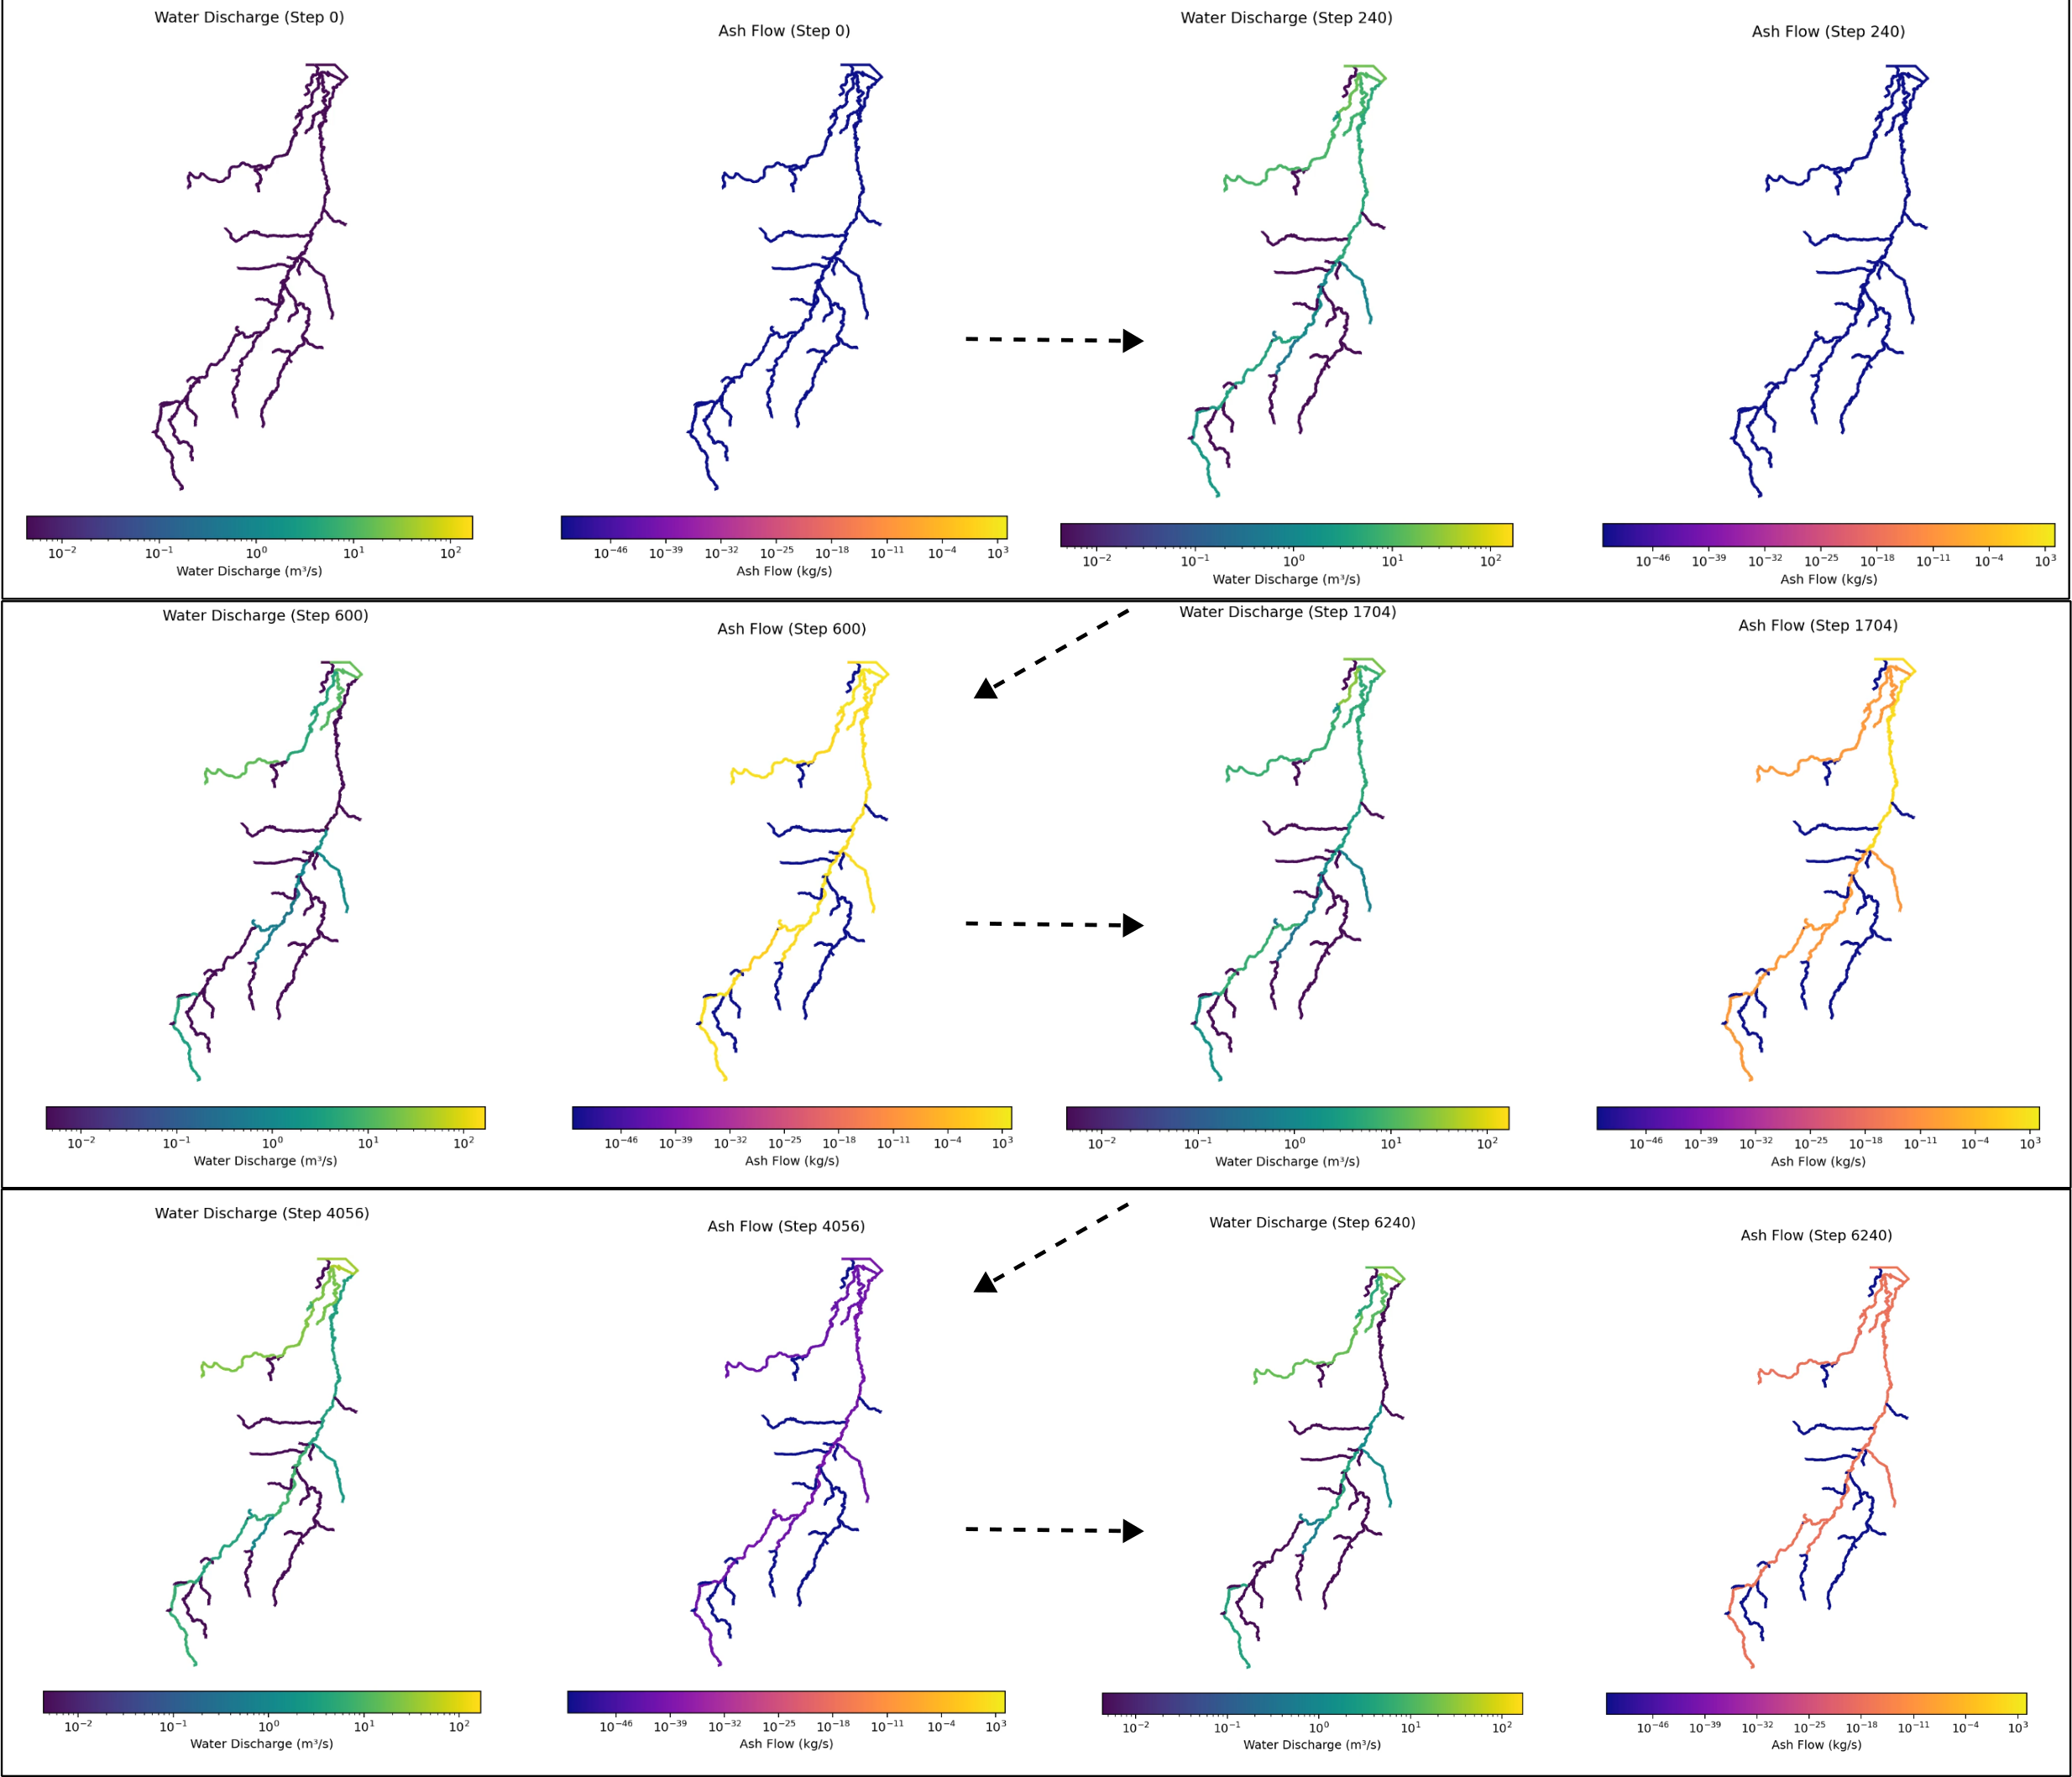
\includegraphics[width=1\linewidth]{animation.png}
    \caption{Snapshots from the network animation showing the spatio-temporal dynamics of the cascade. The left column shows water discharge (m$^3$/s) and the right column shows ash flow (kg/s). \textbf{(a) Step 48 (Day 2):} Baseline conditions. \textbf{(b) Step 528 (Day 22):} Initial mobilization of ash after the first eruption. \textbf{(c) Step 4848 (Day 202):} A major pulse of ash mobilizes throughout the network after the second eruption. \textbf(d) Step 6288 (Day 262): The ash pulse has propagated down the main stem.}
    \label{fig:animation}
\end{figure}


Water discharge is a persistent feature of the network (Fig. \ref{fig:animation}, left column). In contrast, ash flow is highly transient and localized (Fig. \ref{fig:animation}, right column), activated only where there is both available ash and sufficient water flow. The animation stills show the ash pulse being generated in the headwaters (Frame b), propagating through the network (Frame c), and being advected downstream as a concentrated wave (Frame d). This spatio-temporal analysis is crucial for understanding where in the network the greatest hazards (e.g., channel aggradation) might occur at different times during a cascading event.

\section{Discussion}
Our network-based stochastic model serves as a "what-if" virtual testbed, providing new insights into the complex, cascading interactions between volcanic and hydrological hazards. The results not only quantify these interactions but also demonstrate the value of this approach for Disaster Risk Management (DRM) and Climate Change Adaptation (CCA) within a complex multi-risk framework.

The primary contribution of this work is the implementation of a functional virtual testbed for assessing cascading impacts. The model demonstrates that volcanic ash can significantly alter catchment hydrology by reducing infiltration and increasing runoff—a mechanism well-supported by empirical evidence and explicitly implemented via the dynamic Curve Number. Our testbed moves beyond static analysis by simulating the temporal evolution of this risk. It reveals that the period of heightened flood vulnerability can persist for weeks to months, a critical insight for long-term risk management. The analysis explicitly visualizes these cascading effects, showing how the combination of ashfall and extreme precipitation creates compound risks far greater than the sum of their individual parts.

A key objective of virtual testbeds is to support decision-making under uncertainty. Our model achieves this by enabling the systematic exploration of "what-if" scenarios. The virtual testbed allows risk managers to explore low-probability, high-impact events that are absent from historical records but pose a credible threat. The stochastic nature of the model ensures that the outputs are probabilistic, capturing the full range of potential outcomes and helping decision-makers allocate resources effectively to build more resilient communities.

Our framework also provides a direct pathway for integrating Climate Change Adaptation (CCA). The testbed can be readily adapted to explore future conditions by adjusting the parameters of the stochastic precipitation model to align with climate projections. This allows planners to assess how cascading risks might evolve and to develop adaptation strategies that are robust to both current and future climate-influenced hazard regimes.

Finally, while this study focuses on a specific case in New Zealand, its modular, network-based architecture makes our virtual testbed an ideal "building block" for a larger, interconnected digital ecosystem of multi-risk models. This work serves as a practical example of how a standalone testbed can be developed with the principles of interoperability and scalability.

\section{Conclusions}
This study details the conceptualization and implementation of a dynamic, network-based virtual testbed for assessing cascading risks between volcanic ashfall and hydrological systems. By incorporating dynamic temporal processes, our model provides a realistic simulation environment for exploring multi-hazard interactions and their implications for Disaster Risk Management (DRM) and Climate Change Adaptation (CCA).

Our application to the Rangitaiki and Tarawera river systems demonstrates that the testbed can effectively quantify the significant increase in flood risk caused by volcanic ashfall, particularly when compounded with high-intensity precipitation. The ability to run numerous "what-if" scenarios within a stochastic framework provides decision-makers with robust, probabilistic information.

The temporal dynamics captured by the model highlight that risk remains elevated for extended periods post-eruption, a critical consideration for sustained risk management. Most importantly, this work serves as a proof-of-concept for how a virtual testbed can be designed as a modular, transferable building block, offering a promising pathway for bridging the gap between standalone research models and an integrated digital ecosystem of tools designed to help society navigate the challenges of complex, cascading disasters in a changing climate.

\section*{Acknowledgments}
This research was supported by the Resilience to Nature’s Challenges National Science Challenge, funded by the New Zealand Ministry of Business, Innovation and Employment.

\section*{Data Availability}
The model code and simulation configuration files used in this study are available from the corresponding author upon reasonable request.

\bibliography{references}
\begin{thebibliography}{}

\bibitem[Chow et al., 1988]{Chow1988}
Chow, V. T., Maidment, D. R., \& Mays, L. W. (1988). \textit{Applied hydrology}. McGraw-Hill.

\bibitem[De Angeli et al., 2022]{DeAngeli2022}
De Angeli, S., Malamud, B., Rossi, L., Taylor, F., Trasforini, E., \& Rudari, R. (2022). A multihazard framework for spatial-temporal impact analysis. \textit{International Journal of Disaster Risk Reduction, 73}, 102829.

\bibitem[DesInventar, 2023]{DesInventar2023}
DesInventar. (2023). \textit{Sendai framework for disaster risk reduction, Disaster information management system, UNDRR DesInventar Sendai}. Retrieved from www.desinventar.net/what\_is.html.

\bibitem[Dunant et al., 2021a]{Dunant2021a}
Dunant, A., Bebbington, M., \& Davies, T. (2021a). Probabilistic cascading multi-hazard risk assessment methodology using graph theory, a New Zealand trial. \textit{International Journal of Disaster Risk Reduction, 54}, 102018.

\bibitem[Dunant et al., 2021b]{Dunant2021b}
Dunant, A., Bebbington, M., Davies, T., & Horton, P. (2021b). Multi-hazards scenario generator: A network-based simulation of natural disasters. \textit{Risk Analysis, 41}(11), 2154-2176.

\bibitem[Dunant et al., 2025]{Dunant2025}
Dunant, A., Robinson, T. R., Densmore, A. L., Rosser, N. J., Rajbhandari, R. M., Kincey, M., Li, S., Awasthi, P. R., Van Wyk De Vries, M., Guragain, R., Harvey, E., \& Dadson, S. (2025). Impacts from cascading multi-hazards using hypergraphs: A case study from the 2015 Gorkha earthquake in Nepal. \textit{Natural Hazards and Earth System Sciences}, \textit{25}(1), 267–285. \href{https://doi.org/10.5194/nhess-25-267-2025}{https://doi.org/10.5194/nhess-25-267-2025} 

\bibitem[Gill \& Malamud, 2014]{Gill2014}
Gill, J. C., \& Malamud, B. D. (2014). Reviewing and visualizing the interactions of natural hazards. \textit{Reviews of Geophysics, 52}(4), 680-722.

\bibitem[Gonzalez-Mellado \& De la Cruz-Reyna, 2010]{Gonzalez-Mellado2010}
Gonzalez-Mellado, A., \& De la Cruz-Reyna, S. (2010). A simple model for the geometrical description of tephra fall deposits. \textit{Journal of Volcanology and Geothermal Research, 190}(3-4), 317-327.

\bibitem[Gran et al., 2006]{Gran2006}
Gran, K. B., Montgomery, D. R., \& Sutherland, D. G. (2006). Channel bed evolution and sediment transport under declining sand inputs. \textit{Water Resources Research, 42}(10), W10407.

\bibitem[Gran et al., 2011]{Gran2011}
Gran, K. B., Montgomery, D. R., \& Halbur, J. C. (2011). Long-term elevated post-eruption sedimentation at Mount Pinatubo, Philippines. \textit{Geology, 39}(4), 367-370.

\bibitem[Guha-Sapir et al., 2016]{Guha-Sapir2016}
Guha-Sapir, D., Below, R., \& Hoyois, P. (2016). \textit{EM-DAT: The CRED/OFDA international disaster database}. Centre for Research on the Epidemiology of Disasters.

\bibitem[Liu et al., 2016]{Liu2016}
Liu, B., Siu, Y. L., \& Mitchell, G. (2016). Hazard interaction analysis for multi-hazard risk assessment: a systematic classification based on hazard-forming environment. \textit{Natural Hazards and Earth System Sciences, 16}(2), 629-642.

\bibitem[Nairn, 2002]{Nairn2002}
Nairn, I. A. (2002). \textit{Geology of the Okataina Volcanic Centre, scale 1:50 000}. Institute of Geological \& Nuclear Sciences geological map 25.

\bibitem[Pierson \& Major, 2014]{Pierson2014}
Pierson, T. C., \& Major, J. J. (2014). Hydrogeomorphic effects of explosive volcanic eruptions on drainage basins. \textit{Annual Review of Earth and Planetary Sciences, 42}, 469-507.

\bibitem[Tangi et al., 2022]{Tangi2022}
Tangi, M., Bizzi, S., Fryirs, K., & Castelletti, A. (2022). A Dynamic, Network Scale Sediment (Dis)Connectivity Model to Reconstruct Historical Sediment Transfer and River Reach Sediment Budgets. Water Resources Research, 58(2), e2021WR030784. https://doi.org/10.1029/2021WR030784

\bibitem[U.S. Department of Agriculture, 1986]{USDA1986}
U.S. Department of Agriculture, Soil Conservation Service. (1986). \textit{Urban hydrology for small watersheds} (Technical Release 55).

\bibitem[Wilson \& Parker, 1985]{Wilson1985}
Wilson, C. J. N., \& Parker, L. (1985). The Taupo eruption, New Zealand I. General aspects. \textit{Philosophical Transactions of the Royal Society of London. Series A, Mathematical and Physical Sciences, 314}(1529), 199-228.

\end{thebibliography}

\end{document}